\documentclass[a6paper]{article}

\usepackage[total={8.9cm,13cm}, top=.8cm, left=.9cm, includefoot]{geometry}
\usepackage{graphicx}

\usepackage[czech]{babel}
\usepackage[utf8]{inputenc}

\usepackage {abstract}

\newcommand*\podpis{\hspace*{0em plus 1fill}\makebox{..........}}

\newcommand \ukol[1]{
	\item
	#1
	\podpis
}

\renewcommand{\abstractname}{ }

%\pagestyle{empty}
\begin{document}


\author {Anpetu}

\title{\textbf{Akičita čikalan}}
\date{}
\maketitle
\begin{center}
	
{\large
Malý bojovník
}



\vspace{60pt}
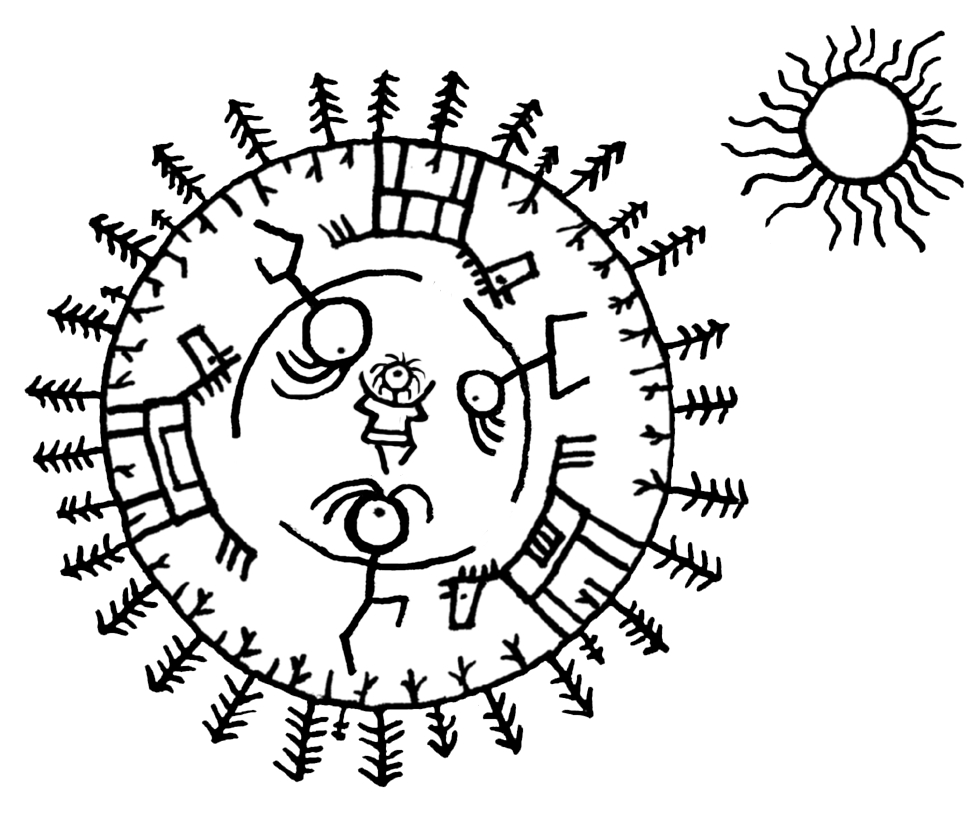
\includegraphics[width=0.6\textwidth]{piktogramy/agles_kluci_kruh.jpg}
\end{center}
\clearpage

\vspace*{15 pt}

\begin{Large}
{Bojovnice, bojovníci,}	
\end{Large}


\vspace{12 pt}
\begin{large}
	
vydali jste se s naším kmenem na dlouhou cestu. Tento sešítek vám bude radit, jaké dovednosti na ní využijete.


\vspace{25 pt}

S vašimi udi budete společně plnit úkoly. U každého splněného úkolu vám uďa podepíše políčko vpravo. 

\end{large}

\clearpage

\section*{Zdatnost} % (fold)
\label{sec:zdatnost}
\begin{itemize}
	\ukol{ Uběhnu 300 m členitým terénem }
	\ukol{ Ušel jsem za jeden den aspoň 12 km }
	\ukol{ Přeskočím svou délku (horizntálně) }
\end{itemize}


% section zdatnost (end)


\section*{Oddíl a skauting} % (fold)
\label{sec:skauting}
\begin{itemize}
	\ukol{ Vím, kdo se zasloužil o vznik skautingu u nás }
	\ukol{ Vím, jak vznikl náš oddíl }
	\ukol{ Byl jsem aspoň na dvou oddílových akcích }
	\ukol{ Znám telefonní číslo na své Uďi }
	\ukol{ Znám oddílový pokřik }
\end{itemize}
% section skauting (end)

\vspace{\fill}

\begin{center}
	
\includegraphics[width=0.3\textwidth]{piktogramy/indos_bezi2.jpg}
\end{center}
\clearpage


\section*{Uzly} % (fold)
\label{sec:uzly}
\begin{itemize}
	\ukol{ Umím si zavázat pohorky }
	\ukol{ Uvážu lodní smyčku }
\end{itemize}
% section uzly (end)


\section*{Tábornictví} % (fold)
\label{sec:tabornictvi}
\begin{itemize}
	\ukol{ S kamarádem dokážu uříznout polínko a rozštípnu ho  }
	\ukol{  Vím, co mám mít na družinovku a celý měsíc jsem nic nezapomněl  }
	\ukol{ Umím si zabalit na vícedenní výpravu sám  }

\end{itemize}
% section tábornictví (end)


\section*{Já a svět} % (fold)
\label{sec:ja_a_sv}
\begin{itemize}
	\ukol{ Zúčastním se dobročinné akce s oddílem.	 }
	\ukol{ Vím, jak se dostat z klubovny domů.	 }
\end{itemize}
% section ja_a_sv (end)


\begin{center}
	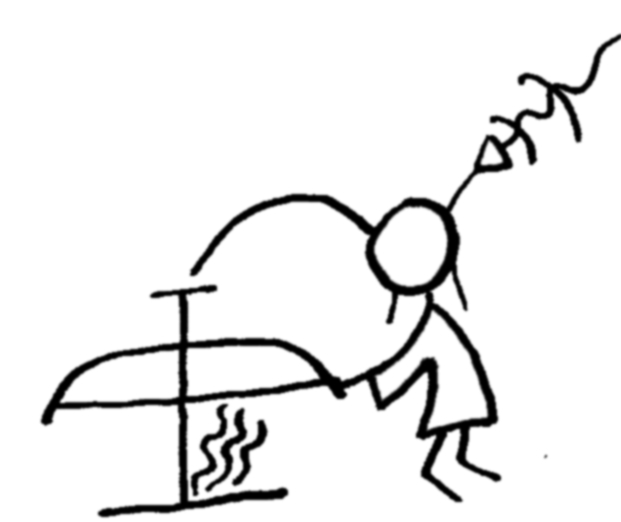
\includegraphics[width=0.35\textwidth]{piktogramy/agles_rozdelava_ohynek.jpg}
\end{center}
\clearpage


\section*{Zdravověda} % (fold)
\label{sec:zdrav}
\begin{itemize}
	\ukol{ Znám čísla IZS	 }
	\ukol{ Vím, co dělat, když se spálím o kamna	 }
	\ukol{ Umím ošetřit rozbité koleno	 }
	\ukol{ Co udělám, když mě bodne vosa? 	 }

\end{itemize}
% section zdrav (end)


\section*{Topografie} % (fold)
\label{sec:topografie}
\begin{itemize}
	\ukol{ Dokážu najít na mapě místo, kde se nacházím. }
	\ukol{ Během jedné výprava si zkusím družinku vést. Nechám si ukázat, kudy půjdeme a potom trasu sleduji.		}

\end{itemize}
% section topografie (end)
\vspace{\fill}
\begin{center}
	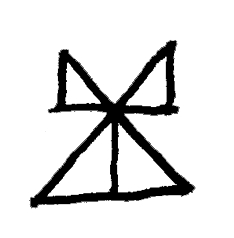
\includegraphics[width=0.25\textwidth]{piktogramy/typka.jpg}
\end{center}
%\vspace{10pt}
\clearpage

\section*{Tvořivost} % (fold)
\label{sec:tvorivost}
\begin{itemize}
	\ukol{ Uvařím čaj z přírodních surovin }
	\item Vyberu si jeden z úkolů:
	\begin{itemize}
		\ukol{ vyřežu něco ze dřeva/kůry }
		\ukol{ složím básničku nebo napíšu svou vlastní pohádku (aspoň 15 vět) }
		\ukol{ upletu si náramek }
		\ukol{ naučím se 3 akordy na kytaru/ukulele }
	\end{itemize}

\end{itemize}
% section tvorivost (end)



\section*{Šifry} % (fold)
\label{sec:sifry}
\begin{itemize}
	\ukol{ Naučím se šifru zvanou mřížka. Dokážu rozluštit zprávu a napsat tři věty.}
	\ukol{ S nápovědou rozluštím zprávu v morseovce, dokážu se morseovkou podepsat.}
\end{itemize}
% section sifry (end)
\vspace{\fill}
\begin{center}
	
\includegraphics[width=0.7\textwidth]{piktogramy/korale.jpg}
\end{center}
\clearpage


\section*{Příroda} % (fold)
\label{sec:priroda}
\begin{itemize}
	\ukol{ Znám 5 jehličnatých a 5 listnatých stromů, vím, jak vypadají a dokážu je určit v přírodě.}
\ukol{ Vyberu si divoké zvíře žijící v ČR, zjistím si o něm informace a povím o něm ostatním.}
\item Vyberu si jeden z úkolů:
\begin{itemize}
	\ukol{ Naučím se poznat 5 stop lesní zvěře. }
	\ukol{ Naučím se poznat  5 divoce rostoucích bylin a vím, na co která pomáhá. }
	\ukol Naučím se rozeznat 5 ptáků podle zpěvu.\podpis

\end{itemize}

\end{itemize}
% section příroda (end)
\vspace{\fill}
\begin{center}
	
\includegraphics[width=0.5\textwidth]{piktogramy/mysicky.jpg}
\end{center}
\clearpage

\vspace*{50pt}
\begin{center}
	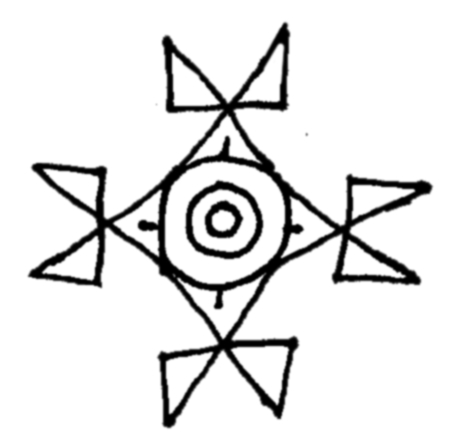
\includegraphics[width=0.5\textwidth]{piktogramy/symbol_kruh_4_typka.jpg}
\end{center}

\vspace{\fill}

\begin{tiny}
	\hspace{\fill}
	Stezky anpetu, V 1.0RC1
\end{tiny}

\end{document}